\begin{frame}
    \begin{exampleblock}{Exercise II}
        \begin{enumerate}
            \item Connect your board, \acs{led} and resistor on your breadboard.
            \item Control the pin connected to the \acs{led} instead of the on-board \acs{led}.
        \end{enumerate}
    \end{exampleblock}
\end{frame}

\begin{frame}{Breadboards}
    \begin{figure}
        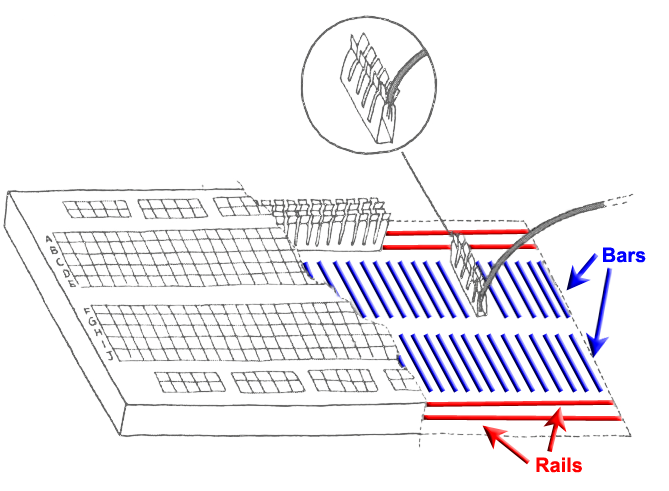
\includegraphics[width=0.9\textwidth]{microcontroller/breadboard-explosion.png}
        \caption{Breadboard connections}
    \end{figure}
\end{frame}

\begin{frame}{\glsentrydesc{led}}
    \begin{figure}
        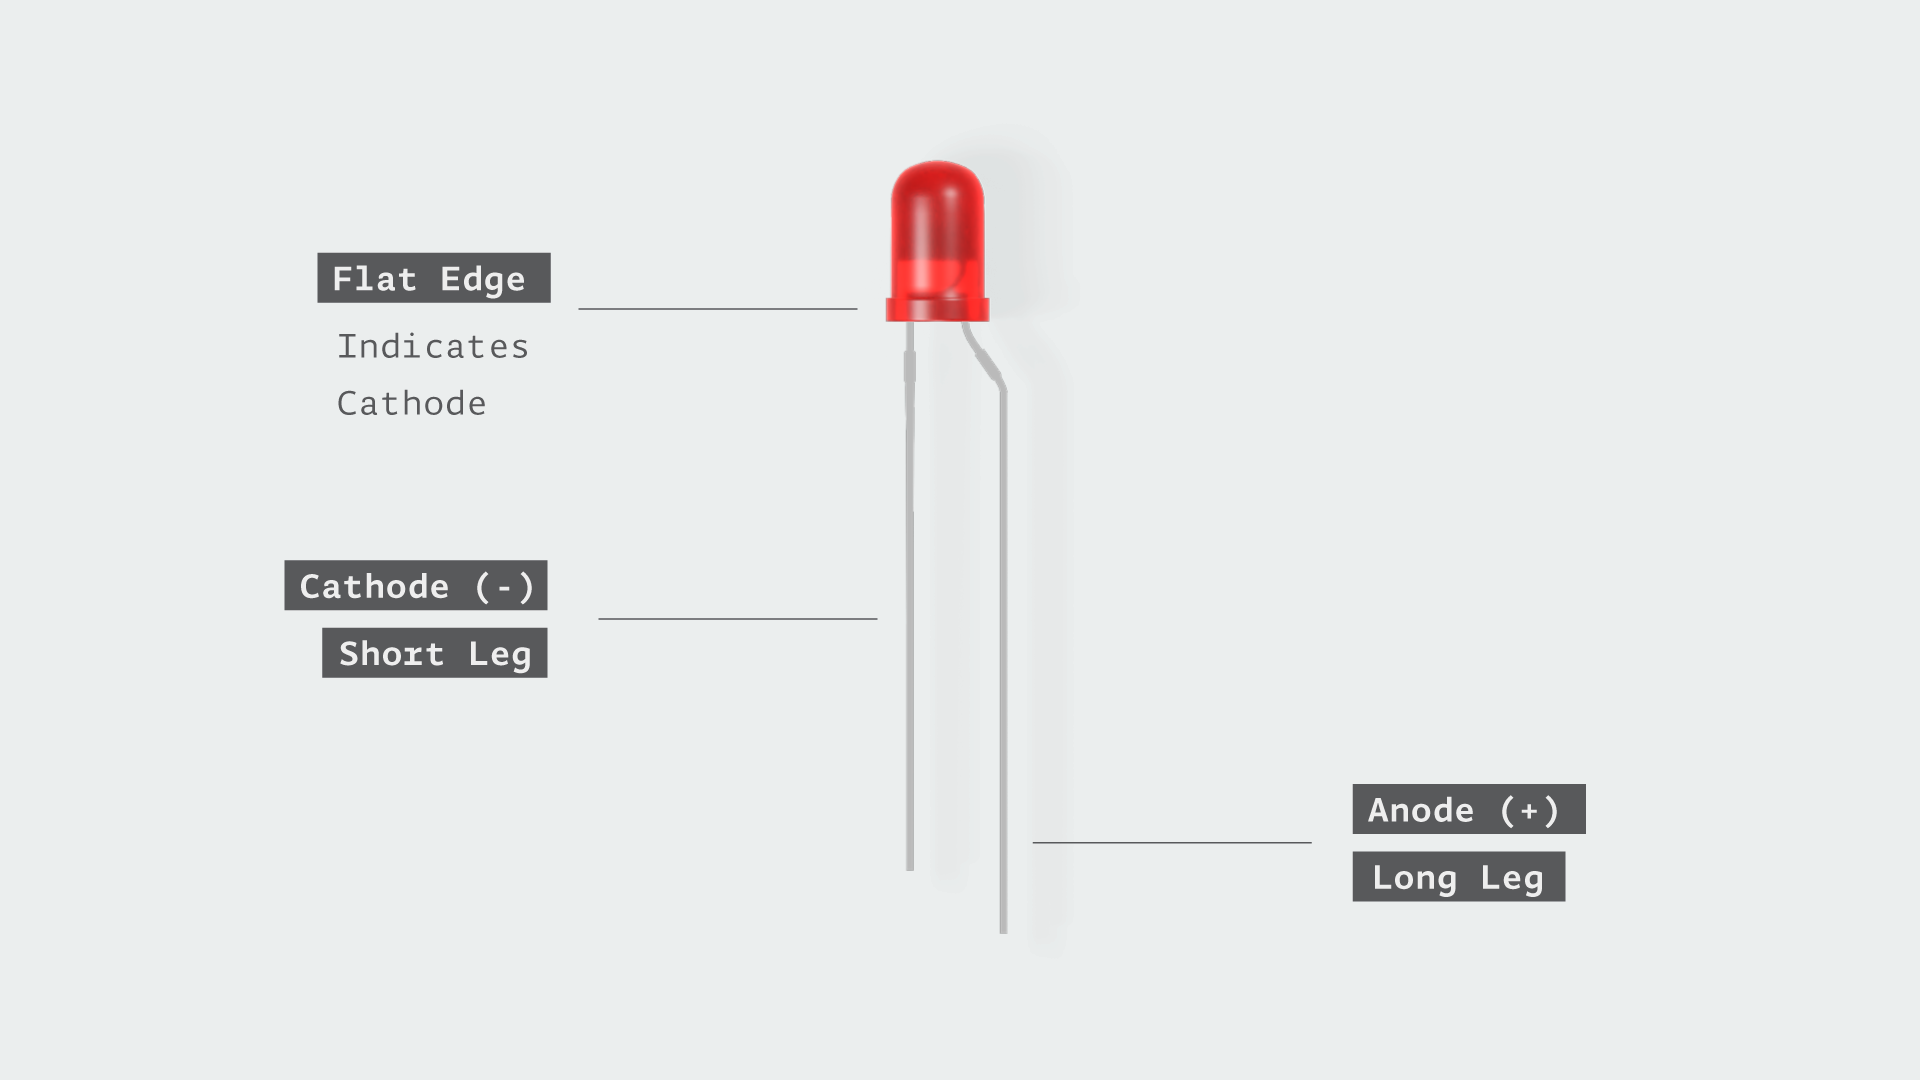
\includegraphics[width=0.9\textwidth]{microcontroller/leds.png}
        \caption{\glsentrytext{led} connections}
    \end{figure}
\end{frame}

\begin{frame}{Resistors}
    \begin{figure}
        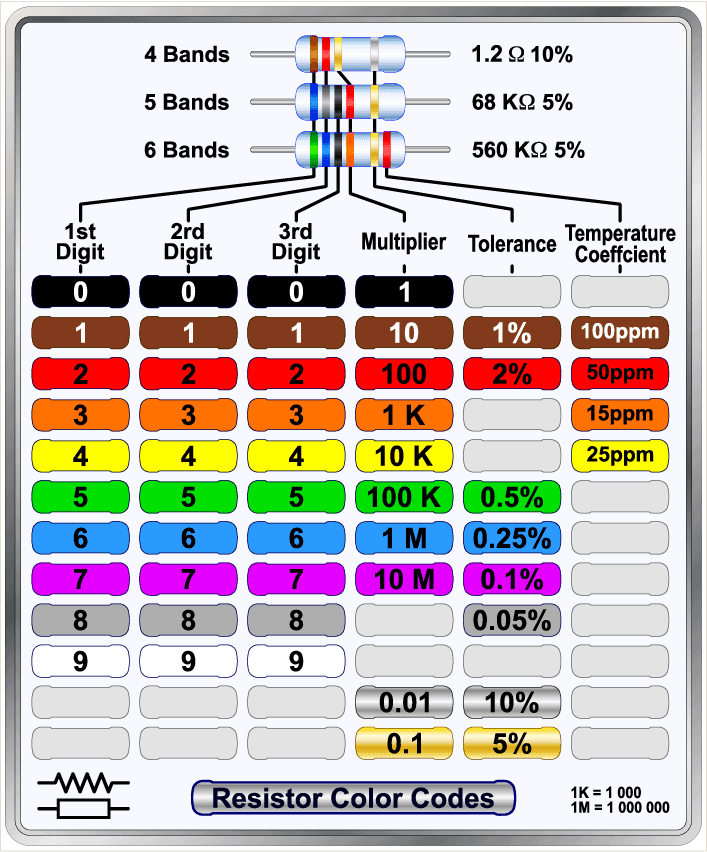
\includegraphics[width=0.55\textwidth]{microcontroller/resistor-color-code.png}
        \caption{Resistors color codes}
    \end{figure}
\end{frame}

\begin{frame}{Solution: Exercise II}
    \begin{listing}[H]
        \inputsource[fontsize=\fontsize{8}{8}]{c}{arduino/blink-external.c}
        \caption{Solution for Exercise II.}
        \label{lst:arduino:exercise:2:solution}
    \end{listing}
\end{frame}

\begin{frame}{Solution: Exercise II}
    \begin{figure}
        \begin{tikzpicture}
            \ctikzset{bipoles/length=1cm, !vi/.style={no v symbols, no i symbols}, bipole voltage style/.style={text opacity=0}, bipole current style/.style={color=ttw-red}}
            \draw (2,4) node[rp2040] (rp20401) {}
            (rp20401.D2) to ++(1,0) to ++(0,4) to ++(2,0) to ++(0,-1) to [R,name=R,l={$R_1 = \SI{220}{\ohm}$},v=$U_1$,voltage shift=3.5,!vi] ++(0,-1) to [leDo,name=LED,l=$D_1$,v=$U_2$,i=$i$,voltage shift=3.5,!vi] ++(0,-2)
            (rp20401.GNDR) to ++(3,0) to ++(0,1);
            \fixedvlen[0.5cm]{R}{$U_1$}[tw-blue]
            \fixedvlen[0.5cm]{LED}{$U_2$}[tw-blue]
            \iarronly{LED}
        \end{tikzpicture}
        \caption{Circuit for Exercise II}
    \end{figure}
\end{frame}

\begin{frame}{Solution: Exercise II}
    \begin{figure}
        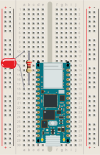
\includegraphics[width=0.35\textwidth]{microcontroller/exercises/exercise-solution-2.pdf}
        \caption{Solution for Exercise II.}
    \end{figure}
\end{frame}